\documentclass{article}
\usepackage{authblk}
\usepackage[utf8]{inputenc}
\usepackage[title]{appendix}
\usepackage{url} % for URLs in references

% Figures and graphics handling
\usepackage{graphicx}
\graphicspath{{./figures/}}

% Page layout, margins, spacing, and line numbers
\usepackage[margin=1in]{geometry}
\usepackage{changepage}
\usepackage{lineno}
\usepackage{setspace}
\linenumbers %Switch command - turn line numbers on/off
\doublespacing %Switch command - set spacing

% Highlighting
\usepackage{xcolor}
\usepackage{soul}

% Package to typset element names efficiently
\usepackage[version=3]{mhchem}

% Work-specific commands - format for SNOwGLoBES, GLoBES, CEvNS, and DukeCEvNS
\newcommand{\cev}{CE$\nu$NS\,}
\newcommand{\snow}{\texttt{SNOwGLoBES}\,}
\newcommand{\glb}{\texttt{GLoBES}\,}
\newcommand{\dukecev}{\texttt{DukeCE$\nu$NS}\,}



% -----------------------------------------------------------------------------------------
% -----------------------------------------------------------------------------------------
% Title, authors and affiliations
\title{\snow: SuperNova Observatories with \glb}

\author[1]{Joshua Albert}
\author[1]{Alex Beck}
\author[1]{Farzan Beroz}
\author[2]{Rachel Carr}
\author[3]{Huaiyu Duan}
\author[4]{Alex Friedland}
\author[5,1]{Nicolas Kaiser}
\author[6]{Jim Kneller}
\author[9]{Elise McCarthy}
\author[1]{Alexander Moss}
\author[7]{Diane Reitzner}
\author[1*]{Kate Scholberg}
\author[10]{Sebastian Torres-Lara}
\author[8]{David Webber}
\author[1]{Roger Wendell}

\affil[1]{Department of Physics, Duke University, Durham, NC 27705}
\affil[2]{Department of Physics, Columbia University, New York, NY 10027}
\affil[3]{Department of Physics, University of New Mexico, Albuquerque, NM, 87131}
\affil[4]{Los Alamos National Laboratory, Los Alamos, NM, 87545}
\affil[5]{Department of Physics, Karlsruhe Institute of Technology, Germany}
\affil[6]{Department of Physics, North Carolina State University, Raleigh, NC,  27695}
\affil[7]{Fermilab, Batavia, IL, 60510-5011}
\affil[8]{Department of Physics, University of Wisconsin, Madison, WI, 53706-1390}
\affil[9]{Department of Physics and Astronomy, University of Rochester, Rochester, NY, 14620}
\affil[10]{Department of Physics, University of Houston, Houston, TX, 77004}
\affil[*]{\textbf{schol@phy.duke.edu}}


\date{\today}

\begin{document}

\maketitle

% -----------------------------------------------------------------------------------------
% -----------------------------------------------------------------------------------------
% BEGIN USER MANUAL TEXT WITH ABSTRACT
% -----------------------------------------------------------------------------------------
\begin{abstract}
This document describes public software for computing interaction rates and distributions of observed quantities for supernova burst neutrinos in common detector materials.  The intent is to provide a very simple and fast data package which can be used to test the observability of physics signatures in current and future detectors, and for evaluation of relative sensitivities of different detector configurations.  The event estimates are made using available cross-sections and parameterized detector responses.  Water, argon, xenon, germanium, scintillator, and lead-based configurations are included. The package makes use of \glb front-end software. \snow is not intended to replace full detector simulations, however output should be useful for many types of studies.  This document serves as a user's manual and provides references for the data files used.
\end{abstract}

% -----------------------------------------------------------------------------------------
% INTRODUCTION TO V. 1.3
% -----------------------------------------------------------------------------------------
\section{Introduction} \label{sec:intro}

A stellar core collapse in the Milky Way or nearby will produce an enormous burst of neutrinos observable in terrestrial detectors.  Such a burst will carry tremendous information about both astrophysics and particle physics: see~\cite{Dighe:2008dq} for recent reviews of physics reach and~\cite{Scholberg:2007nu} for an overview of detection technology.

To enable fast, informative studies of the physics potential of the detection of supernova neutrinos, we have developed \snow, a simple software and database package to compute expected event rates by folding input fluxes with cross-sections and detector parameters.  The output is in the form of interaction rates for each neutrino interaction channel as a function of incident neutrino energy, and ``smeared'' rates as a function of detected energy for each channel (\textit{i.e.} the spectrum that actually be observed in a detector). We have chosen to do the event rate computation using parameterized detector responses, making use of the \glb software~\cite{Huber:2004ka,globes}.  We employ only the front-end rate engine part of \glb, and not the oscillation sensitivity part.
\glb takes as input fluxes, cross sections, ``smearing matrices'' and post-smearing efficiencies.  The smearing matrices incorporate both interaction product spectra and detector response. Fig.~\ref{fig:schematic} gives a schematic overview of the approach.

\begin{figure}
\begin{center}
\includegraphics[height=.3\textheight]{figures/schematic.pdf}
\end{center}
\caption{\snow data flow.}\label{fig:schematic}
\end{figure}

Although with this approach information is lost with respect to a full event-by-event simulation using a neutrino interaction generator and detector simulation (correlations between energy and angle are lost, for example), \snow nevertheless offers a fast, simple method useful for many studies.

\snow should enable studies from differing points of view, by allowing modification of the different kinds of input.  For example:

\begin{itemize}
\item Using the standard cross-sections and detector parameters, a user can study whether specific physics signatures in the fluxes are observable with different detector configurations.

\item Experimentalists can optimize detector configurations by using standard cross-sections and the sample fluxes, and modifying the smearing, efficiency and background files according to different configurations (for example, different PMT coverage in a water Cherenkov configuration).  An early version of \snow was used in this way for the work described in reference~\cite{pwgstudy}.

\item A user could also study systematic errors due to cross-section uncertainties (for example) by comparing event rates computed using cross-sections from different models or with modifications according to estimated uncertainties.

\end{itemize}

Currently, time-dependent fluxes are not supported explicitly, however time dependence can be straightforwardly handled by providing multiple files with fluxes divided into different time bins.

Users should note that \textit{\snow does not employ the oscillation probability and parameter sensitivity computation functionality of \glb at all}.  Although \snow can be helpful for studies of neutrino oscillation by, for example, enabling the comparison of expected  oscillated and non-oscillated fluxes (for oscillation in the supernova progenitor or Earth), the user must compute the oscillation probabilities modulating the flux and evaluate sensitivities separately. \snow is simply an event rate calculator.

Users familiar with version 1.2 will find all functionality they are accustomed to maintained in v.~1.3. Any tools developed for v.~1.2 will require only minimal changes to run with 1.3. Computation speed is identical between versions. However, version 1.3 extends \snow to support low-threshold, low-background liquid noble element dark matter detectors. Version 1.3 offers three new detector materials, flexible energy ranges and binning resolution, a wealth of new supporting code, and significant quality-of-life improvements with new visualization tools and supporting scripts.


% -----------------------------------------------------------------------------------------
% SOFTWARE OVERVIEW - REQUIREMENTS AND INSTRUCTIONS
% -----------------------------------------------------------------------------------------
\section{Software Overview} \label{sec:soft.overview}

% -----------------------------------------------------------------------------------------
\subsection{Dependencies}
\snow v.~1.3 depends on \glb \cite{globes} version 3.0.15 or later (v.~3.1.6 for Mac). The environment variable \texttt{GLB\_DIR} must be set to the \glb installation directory.

\glb itself requires \texttt{Gnu Scientific Library} (\texttt{GSL}), particularly access to the header files. Users of RHEL-derivative Linux distributions such as CentOS and Scientific Linux should be aware that on these operating systems, the \texttt{GSL} header files do not install with the main \texttt{GSL} library. After installing \texttt{GSL} as normal, RHEL-derivative Linux users should install the \texttt{gsl-devel} package to obtain the header files.

\texttt{Perl} is required to execute \snow. The cross-section file, efficiency file, and smearing matrix generation scripts require \texttt{Python}, either 2.6, 2.7, or 3.6+ depending on the script. The most current data visualization tool requires \texttt{Jupyter Notebook}, and some additional sample plotting scripts are available utilizing \texttt{ROOT} \cite{root}. 

The basic \snow install does \textit{not} require \texttt{ROOT}, but advanced users wishing to utilize the \cev-specific extension modules in the \texttt{/smearing\_code/dukecevns/} subdirectory will need \texttt{ROOT} for a majority of the functions. A README and a Makefile are available in this subdirectory with more specific instructions.

% -----------------------------------------------------------------------------------------
\subsection{Download and Installation Instructions}
\begin{itemize}
    \item Version 1.3, the most current release, is available on Github:

\texttt{https://github.com/SNOwGLoBES/snowglobes}

    \item Set the environment variable \texttt{\$SNOWGLOBES} to the directory where \snow will be installed (most commonly \texttt{/home/[user]/snowglobes}).
    \item Set the environment variable \texttt{\$GLB\_DIR} to the location of \glb (most commonly \texttt{/usr/local}).
    \item Go to \texttt{\$\snow/src/} and type \texttt{make}, then \texttt{make install}.
    \item That's it. The now fully-installed package is executed from the \texttt{\$SNOWGLOBES} directory.
\end{itemize}

\subsection{Files}
The \snow package has data files organized into several subdirectories:

\begin{itemize}

\item \texttt{\$SNOWGLOBES/backgrounds} contains the additive background files, labeled by detector configuration.

\item \texttt{\$SNOWGLOBES/bin} contains the \glb executable run by the main script.

\item \texttt{\$SNOWGLOBES/channels} contains the files listing relevant interaction channels for each detector type.

\item \texttt{\$SNOWGLOBES/doc} contains documentation for installation and running, and references for the included data files. 

\item \texttt{\$SNOWGLOBES/effic} contains the post-smearing efficiency files in \glb format, labeled by interaction type and detector configuration. A Python 3.6+ script, written to generate these files for default detector configurations, is located in the main \texttt{\$SNOWGLOBES} directory.

\item \texttt{\$SNOWGLOBES/fluxes} contains the flux files in \glb format, labeled by flux name.

\item \texttt{\$SNOWGLOBES/glb} contains some template files required for building the \glb file.

\item \texttt{\$SNOWGLOBES/out} contains output files generated by \snow, labeled by interaction type and detector configuration, for both interaction rates and smeared rates.

\item \texttt{\$SNOWGLOBES/plots} contains some sample \texttt{Root} plotting scripts. A Jupyter notebook \texttt{Plotter.ipynb}, in the main \texttt{\$SNOWGLOBES} directory, provides additional visualization tools for the channel files, fluxes, smearing matrices, and outfiles.

\item \texttt{\$SNOWGLOBES/smear} contains the smearing matrix files in \glb format, labeled by interaction type and detector configuration. The matrices available on install use the default energy ranges and binning for their interaction type. New smearing matrices generated using the \texttt{create\_smearing\_matrix.py} script are saved here, but will overwrite existing matrices if the user is not careful. To save new smearing matrices without overwriting existing matrices, use the \texttt{\$SNOWGLOBES/smear/new/} subdirectory.

\item \texttt{\$SNOWGLOBES/smearing\_code} contains the \texttt{create\_smearing\_matrix.py} script, which generates new smearing matrices with user-defined parameters (energy ranges, binning resolution, smearing function, etc.) Also located here is the \texttt{/dukecevns/} subdirectory, which is home to the \cev smearing matrix generation code (and a Makefile to compile the \cev code independently of the main \snow library).

\item \texttt{\$SNOWGLOBES/xscns}  contains the cross-section files in \glb format, labeled by interaction channel. Supporting scripts to generate new cross-sections files are located in this directory, in a subdirectory named \texttt{/generic\_xs/}.

\end{itemize}
% -----------------------------------------------------------------------------------------
\subsection{Pre-requisites for Running \snow}

Before running \snow, make sure the following files are made and named appropriately for the detector response you wish to simulate: 
\begin{itemize}
    \item An efficiency file for \textbf{each} interaction in the channel file.  (see Section 7.1)
    \item A cross-sections file for \textbf{each} interaction in the channel file.  (see Section 8.8)
    \item A smearing matrix for \textbf{each} interaction in the channel file. (see Section 9.1 )
\end{itemize}

\noindent If any of these files are missing, \snow will encounter a run error. Supporting scripts are provided for the user to generate any missing files, the details of which can be found in their respective sections. 
% -----------------------------------------------------------------------------------------
\subsection{Running \snow}
The heart of \snow is a script called \texttt{supernova.pl}. This takes four arguments: the run mode, the flux file name, the channel file name, and the experiment configuration name.

\snow is run from the terminal by calling \texttt{supernova.pl} as an executable. The general syntax is

\begin{center}
    \texttt{./supernova.pl [run mode] [flux] [channel file] [experiment name]}
\end{center}

\noindent For example, to compute event rates in the HALO2 detector for the ``Livermore" flux and the interaction channels in \texttt{\$SNOWGLOBES/channels/channels\_lead.dat}, the command will be

\begin{center}
    \texttt{./supernova.pl 0 livermore lead halo2}
\end{center}

The run mode argument specifies the overall state of \snow - to maintain backwards compatibility with the channels available in v.~1.2, run mode 0 specifies \texttt{supernova.pl} should use the v.~1.2 default energy range and binning resolution (incident neutrino energies 0.5-100 MeV, detected energies 0.5-100 MeV, 400 bins in each range). Run mode 1 allows the user to set their own energy range and binning. The \cev interaction channels \textit{require} run mode 1 - for example, a simulation of \cev interactions from the Livermore flux in the \texttt{LUX-ZEPLIN} detector would use the command

\begin{center}
    \texttt{./supernova.pl 1 livermore xenon\_coh lz}
\end{center}

\noindent Users should see Sec.~\ref{sec:run.mode} for more information.

The channel file gives a list of interaction types, a.k.a. ``channels," for which \snow should compute event rates, and the appropriate target weighting factor for each of these channels. Example channel files can be found in the \texttt{\$SNOWGLOBES/channels} subdirectory. The user can modify these to select desired channels or, if \snow is being run in ``new" mode, edit the energy range and binning. See Sec.~\ref{sec:chanfile} for information about the channel file structure, and Sec.~\ref{sec:newstuff} for instructions on adding new channels.

As of v.~1.3, an efficiency file is required to complete a simulation. However, the supporting script \texttt{create\_effc.py} in the top-level \texttt{\$SNOWGLOBES} directory allows the user to set whatever detection efficiency they like, up to and including 100\% detection efficiency at all energies. See Sec.~\ref{sec:bkg&effic} for more information.

Simulation outputs go to the \texttt{\$SNOWGLOBES/out} subdirectory, into spectrum files
named by flux, channel, and experiment configuration. Output text files are generated both for interaction rates (as a function of neutrino energy), and for rates smeared by detector response, as a function of detected energy (the latter are labeled ``\texttt{\_smeared}''). The first column of the output file is energy (either incident neutrino energy in GeV or, for smeared output, detected energy in GeV), and the second column is event rate in that energy bin (events per 0.5 MeV).

Files for which event rates are not weighted by target weighting factor (see Sec.~\ref{subsec:addingchannel}) are labeled ``\texttt{\_unweighted}''. As of \snow version 1.1, the \texttt{supernova.pl} script applies the weighting factors to create the output files.

\texttt{make\_event\_table.pl} is a sample script to return integrated rates for each channel.   It takes the same arguments as \texttt{supernova.pl}; add an additional argument ``1'' if a table of non-smeared rates is desired. As of version~1.3, all outputs can be viewed in the \texttt{Plotter.ipynb} notebook, along with the flux and smearing matrix used in the simulation. Other routines are available - the plotting scripts in the \texttt{\$SNOWGLOBES/plots} directory provide \texttt{Root} examples of handling the output files.

% -----------------------------------------------------------------------------------------
% RUN MODE - flexible binning and changes to supernova.pl
% -----------------------------------------------------------------------------------------
\section{Run Mode}\label{sec:run.mode}

The purpose of the \texttt{run mode} argument is to allow the user to run \snow with either the default v.~1.2 binning parameters or custom binning parameters. The 1.2 defaults are to simulate interactions with incident neutrino energies between 0.5 and 100 MeV, detected energies between 0.5 and 100 MeV, 200 true energy bins and 200 sampling bins per range. For \cev interaction channels, this range is unsuitable. \cev interaction detected energies are $< 10$ keV in xenon; using the default ranges and binning clusters all events in the lowest detected energy bin.

Custom binning, by contrast, can take on whatever values the user prefers. All energy ranges with a low threshold $> 0$ are supported. The authors recommend keeping selected energy ranges close to what is physically anticipated for an interaction channel, but this is not required. In addition, the user may choose to have different numbers of incident and detected energy bins.

To enable users to toggle back and forth between custom binning and default binning (which works well for many supported interaction channels), the \texttt{run mode} argument is called in the command line when a simulation is initiated. \texttt{supernova.pl} knows which channel file format to expect based on the value of \texttt{run mode}:

\begin{adjustwidth}{2cm}{}
    \begin{enumerate}
        \item \texttt{run mode} = 0: default binning parameters
        \item \texttt{run mode} = 1: custom binning parameters
    \end{enumerate}
\end{adjustwidth}

\noindent \textbf{Note:} The user must provide channel files in the correct format for the selected run mode - see Sec.~\ref{sec:chanfile} for details.

% -----------------------------------------------------------------------------------------
% FLUX FILES
% -----------------------------------------------------------------------------------------
\section{Neutrino Fluxes}\label{sec:flux.files}

Two example fluxes are provided with the package: the ``Livermore'' flux~\cite{Totani:1997vj}, and the ``GKVM'' flux~\cite{Gava:2009pj}. Strictly speaking, these are not fluxes but fluences: the flux is integrated over the time of the burst. The spectra for the flavor components of these two example fluences are plotted in Fig.~\ref{fig:fluxes}. We will include more fluxes, and flux generation tools, in the future. The supernova neutrino fluxes are given in units of neutrinos per cm$^{2}$ per energy bin (bin width in GeV) for a supernova occurring 10 kpc away.


\begin{figure}[h]
\includegraphics[height=.3\textheight]{figures/flux_livermore.pdf}
\includegraphics[height=.3\textheight]{figures/flux_gvkm.pdf}

\caption{Left: ``Livermore'' fluence, for different flavor components,
  from reference~\cite{Totani:1997vj}, assuming Fermi-Dirac spectra with
  the average energies indicated as a function of time and zero
  chemical potential, and integrated from $t=0$ to $t=14$~seconds.  Right: ``GVKM'' fluence, integrated over 10
  seconds.}\label{fig:fluxes}
\end{figure}


Also included are fluxes for solar neutrinos. All major solar neutrino components are included (from pp through hep), based on flux shapes from John Bahcall's webpage~\cite{bahcall_webpage}, and magnitudes based on the BS05 (OP)  model~\cite{Bahcall:2004pz}. Mixing is implemented with survival probabilities taken from a figure~\cite{Berryman:2014qha}, and the $\nu_{\mu}$ and $\nu_{\tau}$ probabilities set to be equal. Units of this flux (an actual flux, in this case) are neutrinos/cm$^{2}$/s/0.2~MeV.

In addition to the natural neutrino fluxes, we provide simplified fluxes for debugging purposes. Six monoenergetic fluxes - $1 \times 10^{12}$ $\nu_e$ all arriving with the same incident energy - are provided for incident energies 0.01, 0.02, 0.03, 0.05, 0.075, and 0.1 GeV. These fluxes are intended to verify a given detector configuration is being simulated appropriately.

So long as the units of the flux file are correct, the user may add their own neutrino fluxes locally. These files should be added to \texttt{/snowglobes/fluxes/} with the name \texttt{[flux name].dat} - the \texttt{[flux name]} parameter is the second argument used when running \snow from the command line.


% -----------------------------------------------------------------------------------------
% CHANNEL FILES - LISTS OF INTERACTIONS
% -----------------------------------------------------------------------------------------
\section{Channel Files} \label{sec:chanfile}

The channel file is a list, for a given detector, of the interaction channels \snow should simulate. Channel files are provided on install for most detector configurations in v.~1.3; the user can employ these files as templates to construct their own channel file.

In \snow v.~1.3, the selected run mode impacts the structure of the channel file. For run mode 0, the channel files are structured as in Fig.~\ref{fig:oldsnowchanfile}. The columns are

\begin{adjustwidth}{2cm}{}
    \begin{enumerate}
        \item Interaction type
        \item Interaction number in channel file (indexes from 0)
        \item Neutrino parity
        \item Neutrino flavor
        \item Target weighting factor
    \end{enumerate}
\end{adjustwidth}

\noindent If it does not find this data structure, a 0-mode simulation will terminate unsuccessfully.

In 1-mode simulations, the structure of the channel files is as given in Fig.~\ref{fig:newsnowchanfile}. The columns are

\begin{adjustwidth}{2cm}{}
    \begin{enumerate}
        \item General identifier for \glb postamble file
        \item Interaction type
        \item Interaction number in channel file (indexes from 0)
        \item Neutrino parity
        \item Neutrino flavor
        \item Target weighting factor
        \item Number of incident neutrino flux bins
        \item Low limit of incident neutrino energy [GeV]
        \item High limit of incident neutrino energy [GeV]
        \item Number of detected energy bins
        \item Low limit of detected neutrino energy [GeV]
        \item High limit of detected neutrino energy [GeV]
    \end{enumerate}
\end{adjustwidth}

For \cev interaction simulations, running in 1-mode is mandatory. The default energy range for 0-mode simulations is inappropriate for the energy of the recoiling nucleus in \cev scattering. The energy range bounds in 1-mode are not restricted, but the authors suggest remaining close to what is physically reasonable for your interactions of interest.

\begin{figure}[h]
    \centering
    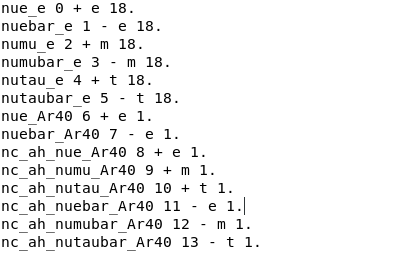
\includegraphics[scale=0.6]{figures/oldSNOWGLOBESchannelfile.png}
    \caption{Example of channel file with default binning}
    \label{fig:oldsnowchanfile}
\end{figure}

\begin{figure}[h!]
\centering
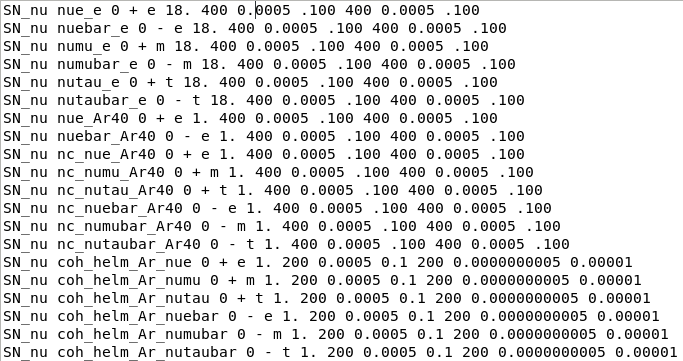
\includegraphics[scale=.4]{figures/newSNOWGLOBESchannelfile.png}
\caption{Example of channel file with custom binning}
\label{fig:newsnowchanfile}
\end{figure}

% -----------------------------------------------------------------------------------------
% DETECTOR CONFIGURATION - FILE AND NAMES PROVIDED ON INSTALL
% -----------------------------------------------------------------------------------------
\section{Detector Configuration} \label{sec:det.config}

The \texttt{detector\_configurations.dat} file contains a list of detectors available to simulate.  The first entry in each row is the detector configuration name. The second entry is the mass in kilotons. The third entry is a target normalization factor - this is
reference targets per amu in the detector material. For example, for water (18 amu per molecule), the reference target is protons, and thus the target normalization factor is $2/18$. For lead, the reference target is \ce{^208Pb}; the target normalization factor is $1/208$.

17 detectors are available on install - for information about adding new configurations to \snow, see Sec.~\ref{sec:newstuff}.

% -----------------------------------------------------------------------------------------
% BACKGROUND AND EFFICIENCY
% -----------------------------------------------------------------------------------------
\section{Detector Background and Efficiency}\label{sec:bkg&effic}

\snow has two mechanisms for the replication of detector effects in its simulation outputs - the detector efficiency file and the background file. The detector efficiency is a \textit{mandatory} simulation component in v.~1.3. The \glb-formatted efficiency files give the detector efficiency as a function of detected energy for a given channel and detector configuration. Generic efficiency files are provided for several detector configurations on install.

When a \snow simulation is initiated, \texttt{supernova.pl} checks the \texttt{\$SNOWGLOBES/effic/[experiment name]} directory for an efficiency file with the name \texttt{effic\_[channel name]\_[experiment name].dat}. It must find one in order to successfully complete a simulation. To help users construct efficiency files of the correct format, we provide the script \texttt{create\_effc.py}. The details of this script are given in Sec.~\ref{subsec:efficsupportscript}.

Unlike the efficiency, including the background in a \snow simulation is optional. The user can provide a file of background events as a function of energy to be smeared by the indicated detector response. This is handled by creating a ``fake'' interaction channel and accompanying smearing file. If a \glb-formatted background file labeled by the detector configuration is present in the \texttt{\$SNOWGLOBES/backgrounds} subdirectory, the background will be smeared and an additional output file created.  The user is responsible for ensuring the background events in the file correspond to the same time interval as the incident neutrino signal.

% -----------------------------------------------------------------------------------------
\subsection{Supporting Script: \texttt{create\_effc.py}} \label{subsec:efficsupportscript}

\texttt{create\_effc.py} is a Python 3.6+ script located in the \texttt{\$SNOWGLOBES} main directory.  It is provided to allow users to readily generate new efficiency files for their detector configuration.

\texttt{create\_effc.py} is executed with the command \texttt{python3.6 [channel file name]}; it then directs the user to identify their detector configuration name. The script matches the configuration name to an efficiency function defined in \texttt{get\_detector\_effic()}. These are detection percentage as a function of detected energy in GeV, defined using lambda functions. 

On install, the efficiency functions are generic - for example, \texttt{create\_effc.py} assumes the \texttt{DarkSide-20k} experiment configuration has a \cev detection efficiency of 0\% for all energies below 50 keV, and 100\% detection efficiency above that threshold. The user can modify the efficiency function locally to more closely mimic their detector behavior.

New efficiency files, one per interaction channel in the channel file, are saved in a \texttt{\$SNOWGLOBES/effic/[detector name]} subdirectory with the format \texttt{effic\_[interaction channel]\_[detector name].dat}. New files will overwrite old ones if a new savepath is not specified.

% -----------------------------------------------------------------------------------------
% CROSS-SECTIONS
% -----------------------------------------------------------------------------------------
\section{Neutrino Interaction Cross-sections}\label{sec:xsecs}
We provide cross-sections relevant for six detector materials relevant for current and near-future detectors: water, scintillator, argon, xenon, germanium, and lead. Distributions of interaction products are taken into account in the ``smearing'' matrices (see Sec.~\ref{sec:smearmatrix}). We expect future upgrades of \snow to incorporate more channels and more materials.

\begin{figure}[htb]
  \centering\includegraphics[width=.75\textwidth]{figures/xscns_water.pdf}
  \caption{Cross sections for relevant processes in water.}
  \label{fig:water_xscns}
\end{figure}

\begin{figure}[htb]
  \centering\includegraphics[width=.75\textwidth]{figures/xscns_scint.pdf}
  \caption{Cross sections for relevant processes in scintillator.}
  \label{fig:scint_xscns}
\end{figure}


\begin{figure}[htb]
  \centering\includegraphics[width=.75\textwidth]{figures/xscns_argon.pdf}
  \caption{Cross sections for relevant processes in liquid argon.}
  \label{fig:argon_xscns}
\end{figure}

\begin{figure}[htb]
  \centering\includegraphics[width=.75\textwidth]{figures/xscns_lead.pdf}
  \caption{Cross sections for relevant processes in lead.}
  \label{fig:lead_xscns}
\end{figure}

% -----------------------------------------------------------------------------------------
\subsection{Inverse Beta Decay}

Inverse beta decay $\bar{\nu}_e+ p \rightarrow e^+ + n$ (IBD) is dominant for detectors with free protons, such as water and scintillator. We use the cross-section from reference~\cite{strumia:2003zx}, plotted in Fig.~\ref{fig:water_xscns}.

% -----------------------------------------------------------------------------------------
\subsection{Neutrino-Electron Elastic Scattering}\label{subsec:nu-e-elastic}

The cross-sections for elastic scattering (ES) of neutrinos on electrons $\nu_{e,x} + e^- \rightarrow \nu_{e,x} + e^-$ (both NC and CC) are known to better than percent level~\cite{Marciano:2003eq}. These cross-sections are plotted in Fig.~\ref{fig:water_xscns}. The electron ES interaction is relevant for all targets, although the scattered electrons may not be observable for some detector configurations (\textit{e.g.} HALO).

% -----------------------------------------------------------------------------------------
\subsection{Interactions with Oxygen}

Interactions on oxygen include the CC interactions $\nu_e+^{16}{\rm
  O}\rightarrow e^-+^{16}{\rm F}$, $\bar{\nu}_e+^{16}{\rm O}
\rightarrow e^++^{16}{\rm N}$.
These interactions have diverse final states, including
ejected nucleons and de-excitation gammas in addition to the produced
lepton.  For the NC interaction with $^{16}$O, $\nu_x+^{16}{\rm O}
\rightarrow \nu_x+ ^{16}{\rm O}^*$, de-excitation gammas are in principle
observable.  We use cross-sections from reference~\cite{Kolbe:2002gk}.
Oxygen cross-sections are plotted in Fig.~\ref{fig:water_xscns}.

% -----------------------------------------------------------------------------------------
\subsection{Interactions with Carbon}

Electron flavor neutrinos will interact with carbon nuclei via the CC interactions $\nu_e+^{12}{\rm C}\rightarrow^{12}{\rm N}+e^-$ and $\bar{\nu}_e +^{12}{\rm C}\rightarrow ^{12}{\rm B}+e^+$. An NC excitation interaction, $\nu_x+^{12}{\rm C}\rightarrow~\nu_x+^{12}{\rm  C}^{*}$ also takes place; this interaction results in a 15.1~MeV de-excitation $\gamma$-ray which can be used to tag this interaction. We use cross-sections from reference~\cite{Kolbe:1999au} for the CC interactions and the measurement from reference~\cite{Armbruster:1998gk} for the NC cross-section. Carbon cross-sections are plotted in Fig.~\ref{fig:scint_xscns}.

% -----------------------------------------------------------------------------------------
\subsection{Charged and Inelastic Neutral Current Interactions with Argon}

We include the CC interactions $\nu_e + ^{40}{\rm Ar} \rightarrow e^- + ^{40}{\rm K^*}$, and $\bar{\nu}_e + ^{40}{\rm Ar} \rightarrow e^+ + ^{40}{\rm Cl^*}$. The cross sections for interactions in argon, from references~\cite{GilBotella:2004bv,Kolbe:2003ys}, are shown in Fig.~\ref{fig:argon_xscns}.   The uncertainties for the recent calculations are at around the 10-20\% level. We have recently added the NC inelastic $\nu_x + ^{40}{\rm Ar} \rightarrow \nu_x+ ^{40}{\rm Ar}^*$ channel, based on private communications with Dr. Anna Hayes.  This interaction is assumed to excite the $^{40}{\rm Ar}$ nucleus to the 9.8~MeV level, from which it will de-excite directly to ground, emitting a 9.8~MeV $\gamma$. The cross sections proved by Dr. Hayes only go up to 52~MeV, so a 2nd order polynomial fit was performed to the provided cross section curve to extrapolate this up to 100 MeV.  The fit was excellent (save the lowest energy point, which was manually fixed), so the extrapolation is likely quite valid.

% -----------------------------------------------------------------------------------------
\subsection{Interactions with Lead}

For lead, we include CC and NC cross-sections for both single and double
neutron ejection channels for:
$\nu_e + ^{208}{\rm Pb} \rightarrow e^- + ^{208}{\rm Bi}^{*}$,
$\nu_x + ^{208}{\rm Pb} \rightarrow \nu_x + ^{208}{\rm Pb}^{*}$,
$\bar{\nu}_x + ^{208}{\rm Pb} \rightarrow \bar{\nu}_x + ^{208}{\rm Pb}^{*}$.

We use cross-sections from~\cite{Engel:2002hg}. Lead cross-sections are plotted in Fig.~\ref{fig:lead_xscns}. Uncertainties on lead cross-sections are evaluated in~\cite{Paar:2011pz}.

% -----------------------------------------------------------------------------------------
\subsection{Coherent Elastic Neutrino-Nucleus Scattering Interactions with Argon, Xenon, and Germanium} \label{subsec:cevxsec}

The \cev interaction channel is new to v.~1.3. First detected by the \texttt{COHERENT} collaboration in 2008 \cite{AGUILARAREVALO200841}, \cev is a weak neutral current interaction which, in liquid xenon, causes interacting nuclei to recoil with $\mathcal{O}(1)$ keV of energy. \cev is flavor-agnostic - detectors sensitive to \cev are equally sensitive to all neutrino flavors. \cev has the highest cross-section of interaction of all neutrino scattering processes.

The \cev cross-section of interaction is given by~\cite{patton_neutrino-nucleus_2012} as:

\begin{equation} \label{eq:dsigma}
    \frac{d\sigma}{dE_R} = \frac{G_F^2}{2 \pi} M \bigg[ 2 - \frac{2E_R}{E_I} + \frac{E_R^2}{E_I^2} - \frac{M E_R}{E_I^2} \bigg] \frac{Q_W^2}{4} \mathcal{F}^2(Q) \times (\hbar c)^{-4}
\end{equation}

\noindent where $G_F$ is the Fermi coupling constant, $M$ the nucleus mass, the weak neutral factor is $Q_W = N - (1-4sin(\theta_W))Z$, and $\mathcal{F}(Q)$ is the nuclear form factor as a function of momentum transfer. The term with the most uncertainty in this expression is the form factor $\mathcal{F}(Q)$, which describes the distribution of nucleons in the target nucleus. A number of expressions for $\mathcal{F}(Q)$ are in use - for example, low-threshold, low-background dark matter experiments tend to prefer the hard-sphere based Helm form factor \cite{lewin_review_1996, akerib_lux-zeplin_2020}:

\begin{equation}
    F(Q) = 3 J_1(Q r_n) \frac{e^{-\frac{(Qs)^2}{2}}}{Q r_n},
    \label{eqn:helmform}
\end{equation}

\noindent while the \texttt{COHERENT} collaboration utilizes the Klein-Nystrand form factor \cite{klein_exclusive_1999}:

\begin{equation}
    F(Q) = 3 \frac{J_1(Q R_A)}{Q R_A} \frac{1}{1+Q^2 a_k^2}.
    \label{eqn:knform}
\end{equation}

\noindent There is no clear consensus which form factor is preferred. To maintain consistency with the internal tools of the most likely users of \snow - low-threshold, low-background dark matter experiments - we have chosen to provide default cross-sections files for natural abundance argon, xenon, and germanium detectors assuming the Helm form factor. As we will explore in Sec.~\ref{subsec:xsecsupportscripts}, the user has the option to change the form factor and abundance locally using a provided cross-section file generation script.

% -----------------------------------------------------------------------------------------
\subsection{Supporting Scripts: Generation of Cross-Sections Files} \label{subsec:xsecsupportscripts}

In the subdirectory \texttt{\$SNOWGLOBES/xscns/generic\_xs}, we provide three scripts to generate new cross-sections files. The first, \texttt{compute\_nu\_e\_cross\_sections.py}, runs with either Python 2.6 and 3.7. It requires no arguments, and generates new cross-sections files for $\nu_{e,x} + e^- \rightarrow \nu_{e,x} + e^-$ ES interactions as detailed in Sec.~\ref{subsec:nu-e-elastic}. This script is most useful in the event a $\nu_{e,x} + e^- \rightarrow \nu_{e,x} + e^-$ ES cross-section file is accidentally deleted, but an experienced user could edit it to change how the cross-section of interaction is calculated.

The \cev cross-sections have a number of parameters the user may wish to change - to that end, we provide \texttt{populate\_CEvNS\_xs.py}. This script is executed using the command \texttt{python3.6 populate\_CEvNS\_xs.py [form factor name]}. Allowable form factor names are Helm and Klein-Nystrand, but space has been designated for future implementation of the Horowitz/numerical and Hoferichter Form Factors. 

By editing the script, the user can change the relative abundance of their detector material. Lines 161, 166, and 171 are lists of relative abundance weights for argon, germanium, and xenon respectively. The weights are arranged from lightest to heaviest isotope. By editing this array, the user can set the relative abundance of their detector material however they like, but care should be taken to ensure the sum of all weights is unity to avoid normalization errors. If the relative abundance is changed here, it must also be changed in the smearing matrices - for more information on that process, see Sec.~\ref{sssec:relabun}.

\texttt{populate\_CEvNS\_xs.py} generates 18 files by default - one cross-section file for each neutrino flavor and element - but the user can limit the script to their material of interest by commenting out the undesirable \texttt{Generate()} calls at the end of the script. To limit the script to a smaller subset of neutrino species, edit the \texttt{neutrinoname} list on line 142.

The final script provided in \texttt{\$SNOWGLOBES/xscns/generic\_xs} is \texttt{universal\_xs.py}. This script will run with either Python 2.7 or 3.7; running the script without arguments will print instructions and produce an example file. This script is designed to assist in adding new interaction channels by producing ``generic" cross-sections files for charged-current interactions on arbitrary nuclei. These generic cross-sections are based on parameterizations of cross-section shape and magnitude. The magnitude parameterization was made by fitting cross sections for various materials provided in \cite{SajjadAthar:2005ke}. The parameterization takes into account the Z (proton number), A (mass number), and Q-value threshold of the reaction.  This parameterization matches the theoretical cross section predictions to within near 20\%, though the theoretical predictions themselves may be far more uncertain than that.

The cross section parameterization is based on the cross sections provided in \snow for deuterium, \ce{^12C}, \ce{^16O}, and \ce{^40Ar}, based on Q-value threshold and mass number. Note that the thresholds used in this parameterization fit may not all be accurate.
While the ground-state to ground-state mass difference (plus electron mass) can be a good estimate for the threshold, the reaction may tend to go to an excited state of the daughter nucleus.

\texttt{universal\_xs.py} comes pre-tuned, although the scripts used for parameterization tuning are provided in \texttt{\$SNOWGLOBES/xscns/generic\_xs/parameterization} if the user wishes to use their own cross sections as input for a new parameterization.  Cross-sections files produced from this script should not be assumed to be accurate.  It is the authors' hope these cross sections are reasonably close (within 50\% or so) to true cross sections, but the model is fairly basic, and the estimates may be off by factors of 5 or more. The cross-sections files from this script should be deployed with caution.

% SMEARING MATRICES
% -----------------------------------------------------------------------------------------
\section{Smearing Matrices} \label{sec:smearmatrix}

\snow uses the smearing matrices to convert incident neutrino energies from the flux file to energies deposited in the detector in the simulation results. These are $i \times j$ comma-delimited matrices, where each matrix entry corresponds to the probability of some incident neutrino energy $j$ causing an interaction in the detector with energy $i$. The probability is convolved with some user-defined smearing function, which mimics reconstruction inaccuracies due to detector effects. When a run of \snow is initiated, \texttt{supernova.pl} searches for a smearing matrix matching the selected detector name, verifies its existence, and then begins the run.

Default smearing matrices are provided on install for most of the default detector configurations, but the user should expect to generate new ones using the provided supporting script.

% -----------------------------------------------------------------------------------------
\subsection{Supporting Script: \texttt{create\_smearing\_matrix.py}} \label{subsec:csm.py}

The script \texttt{create\_smearing\_matrix.py} is provided to generate new smearing matrices according to the user's needs. This script requires Python 3.6 or higher. In the \texttt{\$SNOWGLOBES/smearing\_code} directory, run 
\texttt{python3.6 create\_smearing\_matrix.py} and follow the interactive prompts,
which explain the inputs in detail. The script can also be run with a JSON file as the sole argument.

The script can produce smearing matrices for any of the detector configurations provided on install and the following detector materials:
 
\begin{adjustwidth}{2cm}{}
    \noindent \ce{^16O}, \ce{^12C}, natural abundance \ce{Ar}, \ce{^40Ar}, natural abundance \ce{Ge}, natural abundance \ce{Xe}, \\single-neutron \ce{^208Pb}, double-neutron \ce{^208Pb}
\end{adjustwidth}

\noindent Four interaction mechanisms - neutrino-electron elastic scattering, neutrino-nucleus charged-current scattering, neutrino-nucleus neutral-current scattering, and \cev - are available. It is incumbent on the user to select the appropriate material and interaction mechanism for a given detector type - the script does not prevent the user from generating a smearing matrix which is not correct for their detector configuration. The natural abundance \ce{Ar}, \ce{Xe}, and \ce{Ge} are intended for \cev interaction simulations, and it is possible to modify the relative abundances of these materials - see Sec.~\ref{sssec:relabun} for details. The \ce{^40Ar} material is optimized for the neutrino-nucleus charged-current and neutral-current interactions, but \textit{can} be used for \cev with some modifications to the cross-sections file (see Sec.~\ref{sssec:relabun}).  

Also settable by the user are the energy range of incident neutrinos, energy range of events in detector, and number of bins in each range, a new feature driven by the addition of the \cev interaction channel to v.~1.3. Be aware that when running \texttt{create\_smearing\_matrix.py} the script attempts to match the user-selected energy ranges and binning values to the equivalent parameters in the channel file. The channel file should be edited before \texttt{create\_smearing\_matrix.py} is run.

New smearing matrices generated by \texttt{create\_smearing\_matrix.py} save, by default, into \texttt{\$SNOWGLOBES/smear} where \snow can find them. However, the default smearing matrices provided on install are stored in this directory, and new smearing matrices will overwrite old matrices of the same name. To prevent the default matrices from being overwritten, the user can change the savepath in \texttt{create\_smearing\_matrix.py} - \texttt{\$SNOWGLOBES/smear/new} is recommended for this purpose.

% -----------------------------------------------------------------------------------------
\subsection{\cev Smearing Matrices and the \dukecev Module} \label{subsec:cevnssmearmat}

In the smearing matrix, the probability of an incident neutrino depositing some energy in the detector depends on the differential cross-section of interaction $\frac{d\sigma}{dE_R}$ (see Sec.~\ref{subsec:cevxsec} for discussion of the \cev $\frac{d\sigma}{dE_R}$ expression). $\frac{d\sigma}{dE_R}$ must be separately calculated for each entry in the smearing matrix; the \cev smearing matrices, for the binning suggested on install, are $200 \times 1600$ elements. This computation is entirely too  expensive for \texttt{create\_smearing\_matrix.py} to handle alone. We have chosen to integrate a new submodule, \dukecev, as supporting code for the \cev smearing matrices.

\dukecev is a C++ simulation package. It is capable of rapidly calculating the \cev differential cross-section of interaction for argon, xenon, and germanium, supports user-settable relative abundances, and has three form factors widely in use in the literature - the Helm~\cite{lewin_review_1996}, Klein-Nystrand~\cite{klein_exclusive_1999}, and Horowitz (numerical, data obtained via personal communication) form factors - available for the differential cross-section calculation. \dukecev is also extensible in ways \texttt{create\_smearing\_matrix.py} is not. Available as of 2020 is a form factor based on chiral effective field theory, published by Hoferichter et al. \cite{Hoferichter_2020}; this form factor may capture the structure of target nuclei more accurately than the hard-sphere based Helm or Klein-Nystrand form factors, which will be important for planned comparative studies. The Hoferichter form factor can readily be added to \dukecev by future developers.

In \dukecev, the module \texttt{cevns\_recoil\_response.cc} takes in the detector material (argon, xenon, or germanium, default is natural abundance), desired form factor (default is the Helm form factor), incident neutrino energy range, number of incident energy bins, recoil energy range, and number of recoil bins as inputs. It returns a whitespace-delimited $i \times j$ ``response matrix," where each entry is $\frac{d\sigma}{dE_R}$ for recoil energy $i$ and incident neutrino energy $j$. These response matrices are stored as \texttt{.matrix} files in \texttt{\$SNOWGLOBES/smearing\_code/dukecevns/recoil\_response\_matrices}.

A flowchart of how \cev smearing matrices are built is shown in Fig.~\ref{fig:cevnsmatrixcreation} -  the user interacts exclusively with \texttt{create\_smearing\_matrix.py}. Following the prompts on the terminal, the user selects their detector material, form factor, binning parameters, and the detector resolution function. \texttt{create\_smearing\_matrix.py} takes these inputs and searches the \texttt{/recoil\_response\_matrices/} subdirectory for a response matrix matching the inputs. If it finds one, it reads the file in, transforms the $\frac{d\sigma}{dE_R}$ entries to probabilities, applies the detector resolution function, and saves the resultant smearing matrix to an outfile in \texttt{\$SNOWGLOBES/smear} with the proper format. If it does not find an unsmeared response \texttt{.matrix} file, it directs \texttt{cevns\_recoil\_response} to create one, then performs the above steps on the newly-generated response file.

\begin{figure}[ht]
    \centering
    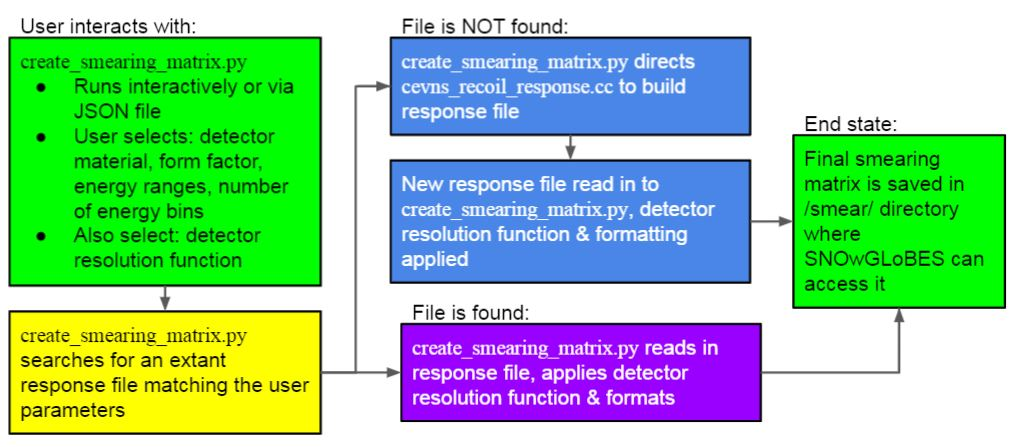
\includegraphics[width=\textwidth,keepaspectratio]{CEvNSmatrixCreationDiagram.JPG}
    \caption{A flowchart of how the \cev smearing matrices are made. The user should never need to interact with any of the \dukecev code; all interactions are done using the \texttt{subprocess} module in \texttt{create\_smearing\_matrix.py}.}
    \label{fig:cevnsmatrixcreation}
\end{figure}

Saving the unsmeared response matrices is a small sacrifice of space - each \texttt{.matrix} file is $\sim 3$ Mb in size - which massively improves the speed at which \cev smearing matrices are generated. It is occasionally necessary to alter the detector resolution function of an existing smearing matrix - with the unsmeared response matrix saved, \texttt{create\_smearing\_matrix.py} does not have to waste time building a new file from scratch for this change.


% -----------------------------------------------------------------------------------------
% HOW TO ADD NEW THINGS
% -----------------------------------------------------------------------------------------
\section{Adding New Stuff} \label{sec:newstuff}

It is straightforward to add new fluxes, channels, targets or detector configurations to \snow.

If you add new data files or configurations, the \snow team would appreciate if you would contact us so that the new information can be made available to all users.

% -----------------------------------------------------------------------------------------
\subsection{Adding New Fluxes}

Fluxes can be added by preparing a file according to the specifications in the \glb manual.  The flux file must be placed in the \texttt{\$SNOWGLOBES/fluxes} directory and named
\texttt{[flux name].dat}. The file should have 501 rows with flux (or fluence) per 0.2~MeV for the different flavors in each row, for neutrino energies ranging from 0.0001 to 0.1001 GeV.

% -----------------------------------------------------------------------------------------
\subsection{Adding New Channels}\label{subsec:addingchannel}

A new channel for a particular material can be added as a new row in the channel file.  Each channel needs a name.  Any text may be used to identify the channel, but we use a channel naming convention as follows: 

\begin{itemize}
    \item  Channels are called \texttt{[neutrino flavor]\_[target name]}, where \texttt{[neutrino flavor]} is \texttt{nue, numu, nutau, nuebar, numubar,} or \texttt{nutaubar}.  If the neutrino target in the detector is a single nuclear isotope, it's written as the element abbreviation followed by the mass number $A$, e.g. \ce{^12C} is rendered C12. An element abbreviation \textit{not} followed by a mass number, e.g. Xe, is assumed to be a mixture of isotopes. For example, the charged current interaction of $\nu_e$ with \ce{^16O} will have the channel name \texttt{nue\_O16}.
    
    \item For inelastic neutral current channels, the channel name is preceded by \texttt{nc\_}. For \cev channels, the channel name is preceded by \texttt{coh\_[form factor name]\_}, where \texttt{[form factor name]} should be \texttt{helm, klein-nystrand}, or \texttt{horowitz}. Note that although neutral current channels (both elastic and inelastic) are flavor-independent, each incoming neutrino flavor must be listed as a separate channel.
    
    \item Specific exclusive final states, such as particular excitations or ejecta, are denoted with a final tag. For example, the neutral current interaction of $\bar{\nu_\mu}$ on \ce{^208Pb} producing double-neutron final states has the channel name \texttt{nc\_numubar\_Pb208\_2n}.
    
    \item The $\bar{\nu}_e+ p \rightarrow e^+ + n$ inverse beta decay channel is an exception to these conventions, and is simply denoted \texttt{ibd}.
\end{itemize}

The format of the channel file is explained in detail in Sec.~\ref{sec:chanfile} - note that two different formatting conventions are in use, depending on whether or not the user wishes to use the default energy ranges and binning parameters.

The target weighting factor - parameter 5 in the channel files for both \snow run modes - requires a bit more explanation; for each material, one selects one target ``reference'' type, for which the weighting factor is unity.  The other targets in the channels file have target weighting factors indicating the relative number of targets per reference target.  For example, for water, we have chosen protons to be the reference target, and inverse beta decay has weighting factor 1. There are 0.5 \ce{^16O} nuclei for each proton, and 5 electrons for each proton in water, so the target weighting factors for elastic scattering on electrons are 5, and for CC and NC interactions on oxygen are 0.5. \cev interactions have a target weighting factor of 1 - the target of a \cev interaction is the nucleus, of which there is 1 per atom.

If you add any new channels to the file, you must provide cross-sections for these channels and put them in the \texttt{\$SNOWGLOBES/xscns} directory.

% -----------------------------------------------------------------------------------------
\subsection{Adding New Detector Configurations}

Each new detector configuration must have smearing and efficiency files associated with it for \textit{each} channel the user wishes to calculate rates for. The smearing and post-smearing efficiency files must be prepared according to the specifications in the \glb manual. In 0 mode, \snow uses 200 true energy bins from 0.0005 to 0.100 GeV and 200 sampling bins over the same range. In 1 mode, the bin numbers and energy range can take on any value desired by the user - to prepare the smearing matrix and efficiency files in 1 mode, first edit the channel file to have the desired energy range and binning parameters. The scripts \texttt{create\_effc.py} and \texttt{create\_smearing\_matrix.py} will query the channel file for the required energy range and binning, then format the new files appropriately.

Smearing matrices must go in the \texttt{\$SNOWGLOBES/smear} directory and be named as follows: \texttt{smear\_[channel name]\_[detector configuration name].dat}. Efficiency files must go in the \texttt{\$SNOWGLOBES/effic/[detector configuration name]} directory and be named as follows: \texttt{effic\_[channel name]\_[detector configuration name].dat}.

% -----------------------------------------------------------------------------------------
\subsection{Adding A New Detector Material}

To add an entirely new detector material, the user must create a new channel file with interaction channels for that material, along with appropriate cross-section files (and a detector configuration employing that material, with requisite efficiency file and smearing matrix).

% -----------------------------------------------------------------------------------------
\subsection{Adding A New Background}

The background calculated by \snow is presumed to be the sum of all relevant backgrounds in the appropriate time interval, as provided by the user.  Backgrounds can be be added by creating a file in the \texttt{backgrounds} subdirectory called \texttt{bg\_[background channel]\_[detector configuration name].dat}. If no file is present in this directory for a given detector configuration, \snow will ignore the background.

An accompanying smearing file must be provided by the user, named \texttt{smear\_[channel name]\_[detector configuration name].dat}. If the background is already smeared, this can be the unit matrix.

% -----------------------------------------------------------------------------------------
\subsection{\cev Parameters}

\cev interactions have a few additional degrees of freedom relative to inelastic NC channels, and can be modified as follows.

% -----------------------------------------------------------------------------------------
\subsubsection{Relative Detector Abundance} \label{sssec:relabun}

The primary detector materials for \cev-sensitive detectors, and the ones supported in v.~1.3 on install, are argon, xenon, and germanium. By default, \snow assumes all three detector materials have natural relative abundances of their constituent isotopes. This is, however, not necessarily true of all future \cev-sensitive detectors. Detectors primarily designed to look for neutrinoless double-beta decay, for example, may have abundances which are far from natural, but they are still capable of potentially detecting a supernova neutrino signal. With an eye to supporting these detectors, we allow the user to specify the isotopic relative abundance of their detector configuration. 

In addition to providing a cross-section file with the desired relative abundance (the process of generating this file is detailed in Sec.~\ref{subsec:xsecsupportscripts}) the user will need to provide an updated smearing matrix.

The \cev smearing matrix code is a module called \dukecev, located in the\\ \texttt{\$SNOWGLOBES/smearing\_code/dukecevns} directory - the directory structure of the important \dukecev files is shown in Fig.~\ref{fig:dukecevstructure}. The relative abundance is defined in the \texttt{mixtures.h} file. In \texttt{mixtures.h}, isotope abundances are defined using the general syntax

\begin{adjustwidth}{2cm}{}
    \texttt{isotopes["element name"].push\_back["isotope"];}\\
    \texttt{molar\_fraction["element name"].push\_back(isotope abundance);}
\end{adjustwidth}

\noindent where the molar fraction being pushed back is the relative abundance of the isotope on the preceding line. Up to four digits of precision are supported for the \texttt{isotope abundance} parameter.

To create, for example, a germanium detector with a 50\% \ce{^70Ge} and 50\% \ce{^73Ge} composition, locate the block where the molecular fractions of the germanium isotopes are defined. Set the molar fractions to zero - \texttt{molar\_fraction["Ge"].push\_back(0)} - for all isotopes \textit{except} \ce{^70Ge} and \ce{^73Ge}. The molar fraction of \ce{^70Ge} and \ce{^73Ge} should be set to 0.5. The code block will look like

\begin{adjustwidth}{2cm}{}
  \texttt{isotopes["Ge"].push\_back("Ge70");}\\
  \texttt{molar\_fraction["Ge"].push\_back(0.5);}\\
  \texttt{isotopes["Ge"].push\_back("Ge72");}\\
  \texttt{molar\_fraction["Ge"].push\_back(0);}\\
  \texttt{isotopes["Ge"].push\_back("Ge73");}\\
  \texttt{molar\_fraction["Ge"].push\_back(0.5);}\\
  \texttt{isotopes["Ge"].push\_back("Ge74");}\\
  \texttt{molar\_fraction["Ge"].push\_back(0);}\\
  \texttt{isotopes["Ge"].push\_back("Ge76");}\\
  \texttt{molar\_fraction["Ge"].push\_back(0);}\\
\end{adjustwidth}

\noindent when complete. Save the edited \texttt{mixtures.h} and, in \texttt{\$SNOWGLOBES/smearing\_code/dukecevns}, type \texttt{make clean}, then \texttt{make}. The \dukecev code will rebuild, and the new abundance will be applied to any germanium smearing matrix generated from that point on. Take care that molar fractions of the new relative abundance sum to 1 - otherwise, you will encounter normalization errors in the smearing matrix. 

Astute users will note there are some monoisotopic detector materials already defined in \texttt{mixtures.h}. To use any of these pre-defined monoisotopic materials, edit line 296 of \texttt{create\_smearing\_matrix.py}, the \texttt{GetTargetName()} function, to add the name of the desired monoisotopic detector material to the dictionary of targets. You can then run \texttt{create\_smearing\_matrix.py} as normal to generate a monoisotopic smearing matrix. New monoisotopic detectors are added by editing \texttt{materials.h} to have the material defined rebuilding \dukecev with \texttt{make clean} and \texttt{make}, and finally adding it as a target to \texttt{create\_smearing\_matrix.py}. Note that the cross-sections file must be edited accordingly in all cases.

Materials beyond argon, xenon, and germanium are available in \texttt{mixtures.h} for future implementation, if desired.

\begin{figure}[h!]
    \centering
    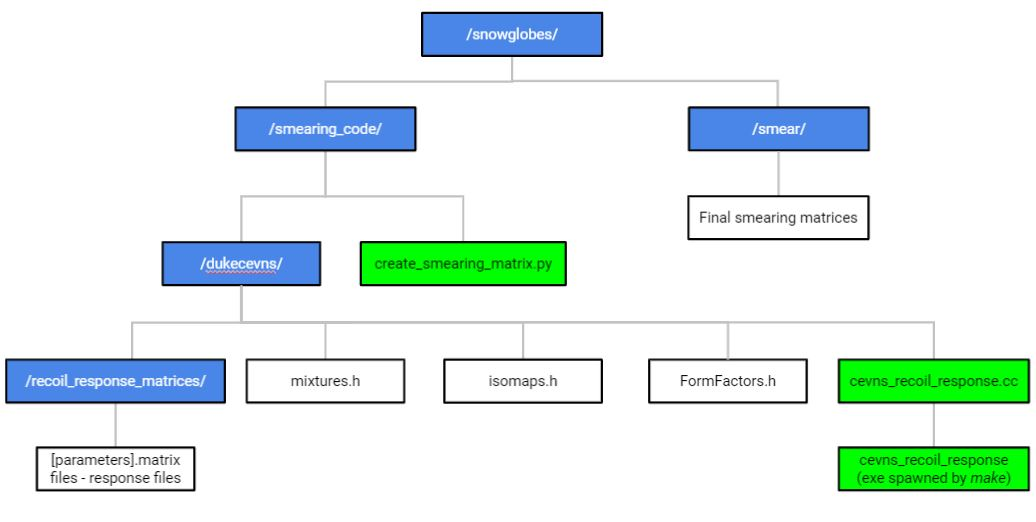
\includegraphics[width=\textwidth]{figures/CodeStructureDukeCEVNS.JPG}
    \caption{The general directory structure of the code used to generate \cev smearing matrices, including \dukecev. Directories and subdirectories are shown in blue, static files are white, and executables are shown in green.}
    \label{fig:dukecevstructure}
\end{figure}

% -----------------------------------------------------------------------------------------
\subsubsection{Form Factors}

New form factors are added to the \dukecev code by first editing \texttt{FormFactors.h} to define the form factor name. Form factors can be provided as closed mathematical expressions (i.e. the Helm and Klein-Nystrand form factors), as numerical parameterization files (i.e. the Horowitz/numerical form factor), or, in the future, as independent code modules which can be imported into \dukecev. The authors recommend this latter approach for the chiral EFT/Hoferichter form factor.

Once the form factor namespace is defined in \texttt{FormFactors.h}, the details of the form factor are defined in \texttt{FormFactors.cc}. Finally, the new form factor must be added as an option in \texttt{cevns\_recoil\_response.cc} - space is designated specifically for the Hoferichter Form Factor on line 313, but other form factors can be added in the same place.

Once all files have been edited and saved, the \dukecev code should be rebuilt by typing \texttt{make clean}, then \texttt{make}. Finally, \texttt{create\_smearing\_matrix.py} should be edited to add the new form factor as an option on line 340 in the function \texttt{GetFormFactorName()}.


% -----------------------------------------------------------------------------------------
\subsubsection{Advanced \cev Modules}

By default, \snow v.~1.3 utilizes only one of several modules available in \dukecev. Located in the same subdirectory are computation routines for simplified supernova neutrino fluxes, \cev interaction rates, and detector responses to simulated events. These are not necessary to run v.~1.3 and, unlike \texttt{cevns\_recoil\_response.cc}, do not compile on install.

A user wishing to develop extended functionality with these routines should utilize the Makefile located in \texttt{/smearing\_code/dukecevns/} to compile the modules independent of \snow. Be aware that the vast majority of these advanced modules require \texttt{ROOT} to compile and run. The \texttt{ROOTSYS} and \texttt{PATH} variables should be set to export in the system \texttt{bashrc} file (or equivalent for non-Linux users) before attempting to compile.


% -----------------------------------------------------------------------------------------
% TO-DO LIST OF FUTURE THINGS TO ADD
% -----------------------------------------------------------------------------------------
\section{Future Upgrades} \label{sec:future}

Several future upgrades are planned for $\snow$:

\begin{itemize}
    \item Inclusion of more targets, channels and fluxes.
    \item As knowledge of detector responses improves (for instance as detector simulation codes improve, and measurements are made) we will update the smearing matrices accordingly.
    \item Computation of angular distributions for channels with asymmetries.
    \item Inclusion of additional cross-sections to allow evaluation of cross-section-related uncertainties.
    \item Addition of frameworks for treatment of time-dependent fluxes, and for treating experimental and theoretical uncertainties.
    \item Expansion of capability to include multiple, distinct backgrounds.
    \item Inclusion of non-supernova fluxes, \textit{e.g.} stopped-pion fluxes.
    \item Additional form factors for \cev channels.
\end{itemize}

Bug reports, suggestions and contributions are very welcome.  Please
contact Kate Scholberg at \texttt{schol@phy.duke.edu}.


% -----------------------------------------------------------------------------------------
% ACKNOWLEDGEMENTS
% -----------------------------------------------------------------------------------------
\section{Acknowledgements}
This work was initiated in the context of the Supernova Burst Physics Topical Group of the
Long Baseline Neutrino Experiment collaboration, for which research activities are primarily supported by the U.S. Department of Energy and the National Science Foundation. AB and NK were supported for work at Duke University by the Deutscher Akademischer Austausch Dienst summer internship program. Development of v.~1.3 was supported by the National Science Foundation `Windows on the Universe: the Era of Multi-Messenger Astrophysics' Program: `WoU-MMA: Collaborative Research: A Next-Generation SuperNova Early Warning System for Multimessenger Astronomy' through Grant Nos. 1914448, 1914409, 1914447, 1914418, 1914410, 1914416, and 1914426. The authors wish to thank the members of the Physics Working Group of the LBNE collaboration, and the Institute for Nuclear Theory at the University of Washington for its hospitality during the summer of 2010.

\begin{appendices}
\section{Change Log}
\begin{itemize}
    \item Version 1.0 is the initial release.
    \item Version 1.1: The target weighting factors are applied automatically by \texttt{supernova.pl}. which creates correctly-weighted output event rate files from the raw unweighted files (the latter now designated unweighted.dat). Example plotting and event table scripts now no longer apply the weighting factor to event rates, and the user is no longer responsible for doing it.
    \item Version 1.2: Capacity for handling backgrounds is added; a single background rate per detector configuration is enabled, if provided by the user. A default background for the \texttt{ar17kt} configuration is included. The NC inelastic interaction cross section is added for \ce{^40Ar}.
    \item Version 1.3: The \cev interaction channel is added for natural abundances of \ce{Ar}, \ce{Xe}, and \ce{Ge} detector materials, with instructions for the user to change the abundance. Detectors utilizing \cev, \cev cross-sections files, and new supporting code are added. User-settable energy ranges and binning resolution is now supported. The efficiency file is now a mandatory simulation component. New output visualization tools are included.
\end{itemize}

\section{GPL}
This program is free software: you can redistribute it and/or modify it under the terms of the GNU General Public License as published by the Free Software Foundation, either version 3 of the License, or (at your option) any later version.

This program is distributed in the hope that it will be useful, but WITHOUT ANY WARRANTY; without even the implied warranty of MERCHANTABILITY or FITNESS FOR A PARTICULAR PURPOSE.  See the GNU General Public License for more details.

You should have received a copy of the GNU General Public License along with this program.  If not, see \texttt{https://www.gnu.org/licenses/}.
\end{appendices}

% -----------------------------------------------------------------------------------------
% -----------------------------------------------------------------------------------------
% -----------------------------------------------------------------------------------------
\bibliography{refs.bib}
\bibliographystyle{unsrt}
 \end{document}
